\subsubsection{Langeweile} \label{langeweile-1}

\todo[inline]{Verantwortlich: Boris\\}

Langeweile wird im Allgemeinen als eine Emotion wahrgenommen, die man erlebt, wenn man einen Zustand durchl{\"a}uft, an dem man kein Interesse hat \cite{vodanovich_2003}. 
Dieses Gef{\"u}hl charakterisiert Inaktivit{\"a}t, Unproduktivit{\"a}t und kann manchmal zu Melancholie oder Traurigkeit f{\"u}hren.
In dieser Studie wird das Erwachen der Langeweile durch eine gr{\"u}ne rotierende Scheibe mit einem schwarzen Strahl verursacht. \\

F{\"u}r das zweite Prototyp wird zwei Szenarios benutzt um die Langweile bei Probanden zu erwecken.
Als ersten wurde eine 5 min{\"u}tigen Video {\"u}ber die "Latente Steuer im Jahres Abschluss" von der Tax Universit{\"a}t benutzt um diese Emotion auszul{\"o}sen. Dabei ging es um eine kurze Einf{\"u}hrungsvideo {\"u}ber Auswirkung von Latentesteuer in der Jahresbilanz. 
Als zweites Szenario w{\"u}rde das "Peg-Turning“ Spiel benutzt. Sein Prinzip besteht darin, eine nach alle 15 Sekunden (oder etwas l{\"a}nger) drehende kreisf{\"o}rmige gr{\"u}ne Scheibe zuzuschauen.


\begin{figure}[H] \centering
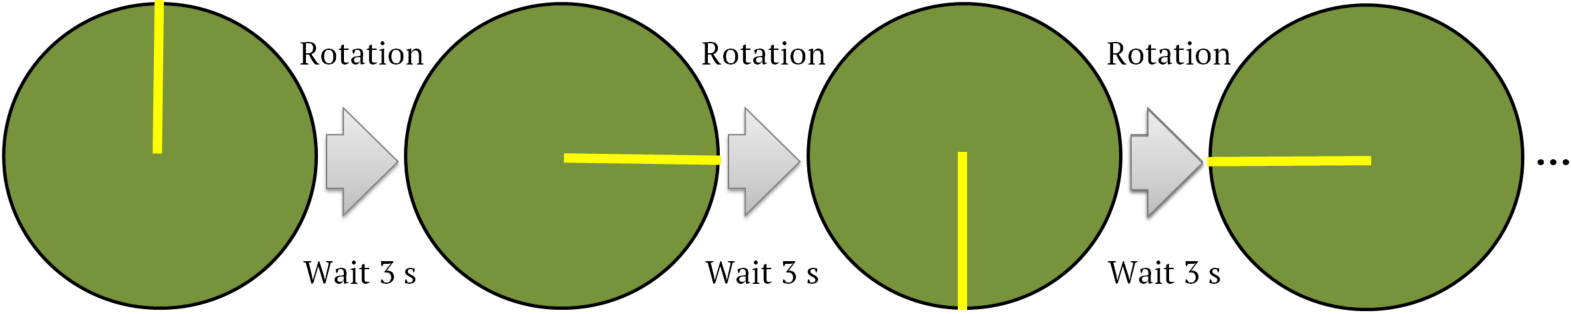
\includegraphics[width=\textwidth]{Images/boredom_game2.png} 
\vspace{-0.3cm} 
\caption{Bild des Langeweile-Szenarios.}
\label{fig-glueck} 
\end{figure}

